% This is samplepaper.tex, a sample chapter demonstrating the
% LLNCS macro package for Springer Computer Science proceedings;
% Version 2.20 of 2017/10/04
%
\documentclass[runningheads]{llncs}
%
\usepackage{graphicx}
\usepackage{multirow}
% Used for displaying a sample figure. If possible, figure files should
% be included in EPS format.
%
% If you use the hyperref package, please uncomment the following line
% to display URLs in blue roman font according to Springer's eBook style:
% \renewcommand\UrlFont{\color{blue}\rmfamily}

%Пакеты для отображения русского шрифта
%\usepackage[utf8]{inputenc}
%\usepackage[russian]{babel}
%Пакеты для гиперссылок
\usepackage{url}
\usepackage{hyperref}
\usepackage{cite}



\begin{document}
%
\title{An Approach for Simultaneous Finding of Multiple Efficient Decisions in Multi-objective Optimization Problems
%with non-convex constraints 
\thanks{This work was supported by the Ministry of Science and Higher Education of the Russian Federation, project no.0729-2020-0055, and by the Research and Education Mathematical Center, project no. 075-02-2020-1483/1.}}
%
\titlerunning{Finding of Multiple Efficient Decisions in MOO Problems}
% If the paper title is too long for the running head, you can set
% an abbreviated paper title here
%
\author{Konstantin Barkalov\orcidID{0000-0001-5273-2471} \and
Victor Gergel\orcidID{0000-0002-4013-2329} \and
Vladimir Grishagin\orcidID{0000-0002-2884-3670} \and
Evgeniy Kozinov\orcidID{0000-0001-6776-0096} 
}
%
\authorrunning{K. Barkalov, V. Gergel, V. Grishagin, E. Kozinov}
% First names are abbreviated in the running head.
% If there are more than two authors, 'et al.' is used.
%
\institute{Lobachevsky State University of Nizhni Novgorod, Nizhni Novgorod, Russia 
\email{\{konstantin.barkalov,evgeny.kozinov\}@itmm.unn.ru,\{gergel,vagris\}@unn.ru}
}
%
\maketitle              % typeset the header of the contribution
%
\begin{abstract}
This paper considers computationally intensive multi-objective optimization problems which require computing multiple Pareto-optimal decisions. It is also assumed that efficiency criteria may be multiextremal, and the cost of calculating function values may be quite high. The proposed approach is based on the reduction of multi-objective optimization problems to one-dimensional global optimization problems that can be solved using efficient information-statistical algorithms of global search. One key innovation of the developed approach consists in the possibility of solving several global optimization problems simultaneously, which allows multiple Pareto-optimal decisions to be obtained. Besides, such approach provides for reuse of the computed search information, which considerably reduces computational effort for solving multi-objective optimization problems. Computational experiments confirm the potential of the proposed approach.

\keywords{Multi-objective optimization \and Multiple global optimization \and Dimensionality reduction \and Optimization method \and Search information \and Computational complexity.}
\end{abstract}
%
%
%
\section{Introduction} \label{sec:01}


Choosing the optimal decisions (decision making) in situations with many different alternatives is a problem that occurs in almost every domain of human activity. In many cases, decision making problems can be viewed as optimization problems of various kinds such as convex programming, discrete optimization, nonlinear programming, etc. In more complex situations, the objective functions that determine the effectiveness of decisions can be multiextremal, and decision making will require solving global optimization problems. In the most general case, however, the effectiveness of decisions may be determined by several objective criteria, which makes it necessary to solve multi-objective optimization (MOO) problems. Thus, MOO problems are the most common decision making statements that one has to solve in many scientific and technical applications. A large number of approaches and methods have been developed to solve such problems and they have been used to solve many decision making problems in various fields of practical applications -- see e.g. \cite{c1,c2,c3,c4,c5,c6,c7,c8,c9}.

One of the approaches most commonly used in the search for efficient decisions is scalarization of the vector efficiency criterion, when a MOO problem is reduced to solving one or several scalar (in the general case, global) optimization problems in which the objective functions are converted to the integrated scalar function. The family of optimization problems generated in such approach is further referred to as multiple global optimization (MGO) problem. Within this approach, we can distinguish lexicographic optimization methods where objective functions are ordered by importance, thus  allowing the optimization of the functions to be carried out sequentially as their importance decreases \cite{c10}. Possible scalarization methods also include various methods of the efficiency criteria convolution such as the weighted sum method, the compromise programming method, the reference point method, the weighted min-max method, etc. -- see, for example, \cite{c2,c11,c12}. 

One common property of methods based on scalarization of the vector efficiency criterion is the existence of some scalarization coefficients that can be varied to obtain different solutions from the Pareto set. Thus, the scalarization coefficients may be interpreted as measures of the importance of the efficiency criteria determined by the decision maker (DM) according to his/her perception of the required optimality of the decisions to be made. As a result, the general scheme for solving the MOO problem can be represented as a sequence of steps; at each step, DM sets the necessary scalarization coefficients, then the resulting scalar optimization problem is solved, after that DM analyzes the efficient decision found and, if necessary, the above steps are repeated.

The general scheme discussed above can be extended by the possibility of selecting not one but several different scalarization coefficient options at each step. With this possibility, the task of coefficient assignment becomes less complex for DM. Solving several generated scalar optimization problems simultaneously allows one to get efficient decision estimates at the very early stages of computations thus making it possible to change dynamically (in the process of computations) the set of problems being solved: to stop solving obviously unproductive (from DM's point of view) ones or to add new optimization problems.

It is also important to note that by solving simultaneously a large number of scalar optimization problems thus generated it is possible to significantly decrease computational complexity of each separate problem. This effect is achieved due to the fact that all such scalar problems  are based on the same MOO problem and, consequently, all computed values of the efficiency criteria of the MOO problem can be reduced to values of any scalar problem being solved simultaneously without any time consuming calculations. In such cases, all the search information obtained in solving any single scalar problem can be used for solving all other scalar problems of the same set. 

This paper presents the results of the authors' continuing research aimed to develop efficient methods for solving MOO problems \cite{c35,c36,c37,c44}. In \cite{c35}, some methods for solving global optimization problems are considered, in \cite{c36},  a general decision-making model based on MOO problems is proposed, and in \cite{c37}, a theoretical analysis is presented regarding the effectiveness of the use of search information when solving MOO problems. In \cite{c44}, we consider MOO problems in which the efficiency criteria can be ordered by importance (lexicographic multi-objective optimization). In this case, MOO problems are reduced to global optimization problems with non-convex constraints for which constrained optimization methods should be applied. In this paper, we propose new computational schemes for using search information that significantly reduce the amount of calculations required to solve MOO problems.

The structure of the paper is as follows. In Section \ref{sec:02}, we give the statement of the multi-objective optimization problem. Section \ref{sec:03} presents a scheme for reduction of multi-objective optimization problems to one-dimensional global optimization problems as well as some methods for solving such problems. Section \ref{sec:04} considers the proposed approach for simultaneous solution of several global optimization problems yielding several Pareto-optimal decisions at a time. Section \ref{sec:05} contains the results of numerical experiments confirming the effectiveness of the proposed approach. In conclusion, the results obtained are discussed and possible main directions of further research are outlined.


\section{Problem statement} \label{sec:02}

In the most general form, the MOO problem can be formulated as follows
\begin{equation}
\label{eq:01}
f(y) = (f_1(y), f_2(y), \dots, f_s(y)) \to \min,  y\in D,
\end{equation}
where $f(y) = (f_1(y), f_2(y), \dots, f_s(y))$ are objective functions (efficiency criteria), $y = (y_1, y_2, \dots , y_N)$ is the vector of varied parameters, and $N$ is the dimensionality of the multi-objective optimization problem to be solved. The set of possible parameter values (search domain) $D$ is usually an $N$-dimensional hyperinterval
\begin{equation}
\label{eq:02}
D  = \{ y\in R^N: a_i \leq y_i \leq b_i, 1 \leq i \leq N \}
\end{equation}
for given boundary vectors $a$ and $b$.

Without loss of generality, it is assumed that objective functions should be minimized to improve the decision efficiency $y \in D$. It is also assumed that $f_i(y)$, $1 \leq i \leq s$, are multiextremal and have the form of time-consuming ``black-box'' computational procedures. It is also assumed that the objective functions $f_i(y)$, $1 \leq i \leq s$, satisfy the Lipschitz condition 
\begin{equation}
\label{eq:03}
|f_i(y') - f_i(y'')| \leq L_i\|y' - y''\|, y', y'' \in D, 1 \leq i \leq s,
\end{equation}
where $L_i$, $1 \leq i \leq s$, are the Lipschitz constants and $\|*\|$ denotes the Euclidean norm in $R^N$.  Condition (\ref{eq:03}) means that for variations of the parameter $y \in D$, the corresponding changes in the values of the functions $f_i(y)$, $1 \leq i \leq s$, are bounded. 

\section{Reducing the Problem of Multi-objective Optimization to the Problems of One-dimensional Global Optimization} \label{sec:03}

As mentioned earlier, in the framework of the proposed approach the solution of MOO problems is reduced to solving one or several scalar global optimization problems in which a single efficiency criterion is generated using some scalarization methods of multiple objective functions. Below, we consider a general scheme for such reduction of the MOO problem and present a method for solving the generated global optimization problems.

\subsection{Scalarization of multiple objective functions}
\label{subsec:31}
 
In the most general form, the global optimization problem generated by the scalarization of multiple objective functions of the MOO problem can be represented in the form
\begin{equation}
\label{eq:04}
\min_{y \in D} {\varphi(y)} = \min_{y \in D} F(\lambda, y),
\end{equation}
where $F$ is a scalar multiextremal function generated as a result of scalarization of objective functions $f_i$, $1 \leq i \leq s$, $\lambda$ is the vector of parameters of the applied convolution of functions, and $D$ is the search domain from (\ref{eq:01}). In the proposed approach, we use for scalarization the compromise programming method \cite{c2,c11}, where solution of the MOO problem consists in finding the efficient decision corresponding most closely to the values of the objective functions of the specified reference decision $y^0 \in D$. In this case, a possible statement of scalar optimization problem can have the form 
\begin{equation}
\label{eq:05}
\min_{y \in D} F(\lambda,y)=\min_{y \in D} \left\{ \frac{1}{s} \sum_{i=1}^s {\lambda_i (f_i (y)-f_i (y^0 ))^2} \right\},
\end{equation}
where $F(\lambda,y)$ is the standard deviation of the values of the objective functions $f_i$, $1 \leq i \leq s$, for the decision $y \in D$ and for the specified reference decision $y^0 \in D$, while the coefficients $\lambda_i$, $0 \leq \lambda_i \leq 1$, $1 \leq i \leq s$, are measures of the importance of the approximation accuracy for each variable $y_i$, $1 \leq i \leq N$, separately. Without loss of generality, we can assume that the domain of possible values of the coefficients $\lambda$ is a set 
\begin{equation}
\label{eq:06}
\lambda=(\lambda_1,\lambda_2, \dots, \lambda_s)\in \Lambda \subset R^s: \sum_{i=1}^{s}\lambda_i=1, \lambda_i \geq 0, 1 \leq i \leq s.
\end{equation}

The reference decision $y^0 \in D$ in (\ref{eq:05}) can be known \textit{a priori} or determined on the basis of some known prototype. In many cases, an abstract ideal decision $y^0 \in D$ is used as the reference decision $y^*\in D$ in which the objective functions $f_i$, $1 \leq i \leq s$, have minimal possible values, i.e.
\begin{equation}
\label{eq:07}
f_i^* =f_i (y^*)=\min_{y \in D} f_i (y), 1 \leq i \leq s.
\end{equation}

Note that by virtue of (\ref{eq:03}) the scalar function $F(\lambda,y)$ from (\ref{eq:05}) also satisfies the Lipschitz condition with some constant $L$, i.e.
\begin{equation}
\label{eq:08}
|F(\lambda, y') - F(\lambda, y'')| \leq L\|y' - y''\|, \; y',y''\in D.
\end{equation}

\subsection{Dimensionality reduction} 
\label{subsec:32}

As already mentioned, problem (\ref{eq:04}) is a multidimensional global optimization problem. Problems of this kind are computationally complex and are known to be subject to the ``curse of dimensionality'' -- computational complexity increases exponentially with increasing dimensionality of the optimization problem being solved \cite{c13,c14,c15,c16,c17,c18,c19,c20}. Nevertheless, the computational complexity of global optimization algorithms can be significantly reduced by dimensionality reduction based on the use of a Peano space-filling curve (or evolvent) $y(x)$ that uniquely and continuously maps the segment $[0,1]$ on an $N$-dimensional domain $D$ -- see, for example, \cite{c15,c21}. As a result of such reduction, multidimensional global optimization problems (\ref{eq:04}) are reduced to one-dimensional problems
\begin{equation}
\label{eq:09}
\min_{x \in [0,1]} \varphi (y(x))= \min_{y \in D} \varphi(y).
\end{equation}

The resulting one-dimensional functions $\varphi(y(x))$ satisfy the uniform H{\" o}lder condition, i.e.
\begin{equation}
\label{eq:10}
|\varphi (y(x'))- \varphi (y(x''))| \leq H |x'-x''|^{1/N}, \; x',x''\in[0,1],
\end{equation}
where the constant $H$ is defined by the relation $H=2L\sqrt{N+3}$, $L$ is the Lipschitz constant from (\ref{eq:08}), and $N$ is the dimensionality of the MOO problem (\ref{eq:01}). 


\subsection{Solving the one-dimensional reduced optimization problem} 
\label{subsec:33}

Using the dimensionality reduction results in one more additional advantage of the proposed approach: many well-known one-dimensional global search algorithms (possibly, after some additional generalisation) can be used to solve the initial multidimensional MOO problem from (\ref{eq:01}) \cite{c22,c23,c24,c25,c26,c27,c28,c29}. At the same time, it should be noted that most works where dimensionality reduction is a key feature for solving multiextremal problems like (\ref{eq:04}) rely on the information-statistical theory of global search \cite{c15}. This theory has provided the basis for developing a large number of efficient methods for multiextremal optimization \cite{c28,c29,c30,c31,c32,c33,c34,c35,c36,c37}.

Within the framework of information-statistical theory, a general computational scheme of global optimization algorithms was proposed which in brief is as follows \cite{c15,c30,c35}.

Let $k$, $k \geq 2$, global search iterations aimed to minimize the function $\varphi(y(x))$ from (\ref{eq:09}) were completed. Then, to perform adaptive choice of the points of next iterations, the optimization algorithm estimates the possibility that the global minimum is located  in the intervals, into which the initial segment $[0,1]$ is divided by the points of earlier global search  iterations
\begin{equation}
\label{eq:11}
x_1<x_2< \dots <x_k.
\end{equation}

This estimate is determined by means of characteristics $R(i)$ of intervals $(x_{i-1},x_i)$, $1 < i \leq k$, whose values should be proportional to the degree of possibility that the global minimum is located  in these intervals. The type of these characteristics depends on the global optimization algorithm used -- thus, for example, for an algorithm which constructs a uniform dense grid in the global search domain, the characteristic is simply the interval length 
\begin{equation}
\label{eq:12}
R(i)=(x_i-x_{i-1}), 1 < i \leq k.
\end{equation}


For the algorithms proposed in \cite{c22,c23}, when dimensionality reduction is applied, the characteristic is an estimate of the minimum possible value of the function $\varphi(y(x))$ to be minimized on the interval $(x_{i-1},x_i )$, $1 < i \leq k$, i.e.
\begin{equation}
\label{eq:13}
R(i) = 0.5 H \rho_i - 0.5 (z_{i-1} + z_i ), \rho_i = (x_i-x_{i-1} )^{1⁄N}, 1 < i \leq k,
\end{equation}
where $H$ is the H{\" o}lder constant from (\ref{eq:10}) for the reduced global optimization problem being solved (\ref{eq:09}), $z_i = \varphi(y(z_i))$, $1 \leq i \leq k,$ and $N$ is the dimensionality of the problem from (\ref{eq:01})).  For the global search algorithm (GSA) \cite{c15,c24} developed in the framework of the information-statistical approach, the characteristic is
\begin{equation}
\label{eq:14}
R(i)=m\rho_i+\frac{(z_i-z_{i-1})^2}{m\rho_i}-2(z_{i-1}+z_i ),\rho_i=(x_i-x_{i-1})^{1/N}, 1 < i \leq k,
\end{equation}
where $m$ is a numerical estimate of the H{\" o}lder constant derived from available search information
\begin{equation}
\label{eq:15}
m= r M, M = \max \{ |z_i-z_{i-1} | ⁄ \rho_i, 1 < i \leq  k \}
\end{equation}
 ($r>1$ is a parameter of the GSA algorithm).

The presence of interval characteristics makes it possible to describe the procedure of global search iteration as the following sequence of steps \cite{c15}.

\textit{Step 1.} Calculate characteristics of the  intervals $R(i)$, $1 < i \leq k$, and determine the interval with the maximum characteristic
\begin{equation}
\label{eq:16}
R(t) = \max \{ R(i), 1< i \leq k \}.
\end{equation}

\textit{Step 2.} Select the next iteration point in the interval with the maximum characteristic
\begin{equation}
\label{eq:17}
x^{k+1}=X(x_{t-1}, x_t)\footnote{The rule $X$ for selecting the point $x^{k+1}$ of the next iteration in the interval $(x_{t-1}, x_t)$ is stated by the global optimization algorithm},
\end{equation}
calculate the value $z^{k+1}$ of the function to be minimized at this point (the procedure for calculating the function value will be further referred to as a trial).

\textit{Step 3.} Check the stopping condition
\begin{equation}
\label{eq:18}
\rho_t \leq \varepsilon,
\end{equation}
where $\rho_t = (x_t-x_{t-1})^{1⁄N}$, $t$ is from (\ref{eq:16}) and $\varepsilon > 0$ is the specified accuracy of the solution. If the stopping condition (\ref{eq:18}) is met, then the solving of the optimization problem is stopped, otherwise $k=k+1$ is assumed and the next global search iteration begins.

After completing the calculations, the lowest computed value of the function being minimized can be taken as the global minimum estimate
\begin{equation}
\label{eq:19}
z_k^* = \min \{ z_i, 1 \leq i \leq k\}.
\end{equation}

It should be noted again that the computational scheme discussed above is quite general. Many global search algorithms can be represented within this scheme, as evidenced, in particular, by examples (\ref{eq:12})--(\ref{eq:14}) and other global optimization algorithms -- see, for example, \cite{c28,c29,c30,c31,c32,c33,c34,c35,c36,c37}. 

Convergence conditions of the algorithms are formulated in the form (\ref{eq:16})--(\ref{eq:18}) depend on the properties of the interval characteristics used. One of sufficient conditions for convergence of algorithms is, for example, the requirement that the characteristic of the interval containing the global minimum point should take on the maximum value at step 1 of the scheme (\ref{eq:16})--(\ref{eq:18}) during the global search iterations. This condition is satisfied, for example, for the multidimensional generalized algorithms proposed in \cite{c22,c23} when the H{\"o}lder constant from (\ref{eq:10}) is specified exactly. For GSA, a sufficient condition for convergence is the relation 
\begin{equation}
\label{eq:20}
m \geq 2^{3-1⁄N} L\sqrt{N+3},
\end{equation}
which must be fulfilled starting from some iteration $k>1$ of the global search ($L$ is the Lipschitz constant from (\ref{eq:08})) \cite{c15}. Moreover, if condition (\ref{eq:20}) is satisfied, only the points of the global minimum of the function $\varphi(y)$ from (\ref{eq:04}) will be the limit points of the trial sequence $\{y^k=y(x^k)\}$ generated by the GSA algorithm.

\section{An Approach for Simultaneous Finding of Multiple Efficient Decisions in Multi-objective Optimization Problems} \label{sec:04}

In this Section, the proposed approach for finding $p$, $p>1$ Pareto-optimal decisions of the MOO problem is presented. This problem is formulated as the problem of solving the set $\Phi_p (y)$, $p>1$ of global optimization problems (see \ref{subsec:41}). To solve this set of optimization problems, two efficient computational schemes are proposed. The first scheme is based on the traditional sequential procedure for solving multiple problems, however, to solve each subsequent optimization problem, all the search information obtained during previous calculations is taken into account. This accumulated search information can significantly reduce the number of global search iterations required to solve the next optimization problems of the set $\Phi_p (y)$ (see \ref{subsec:42} and Section \ref{sec:05}). In the second scheme, all the problems of the set $\Phi_p (y)$ are solved simultaneously, but the search information obtained when solving each problem is also used for solving all the other problems of the set $\Phi_p (y)$ (see \ref{subsec:43}). This useful exchange of search information also significantly reduces the amount of required calculations for solving the problems of the set $\Phi_p (y)$.

\subsection{The need to solve multiple global optimization problems} 
\label{subsec:41}

As mentioned earlier, in the process of solving the MOO problem, it may be necessary to find several different efficient decisions due to possible changes in the optimality requirements. Obtaining different efficient decisions in the proposed approach is achieved by choosing different convolution coefficients (importance indicators) for the objective functions $f_i(y)$, $1 \leq i \leq s$, which results in obtaining different  scalar multiextremal functions $F(\lambda, y)$ from (\ref{eq:04}). These functions $F(\lambda, y)$ can be optimized sequentially. This determines a multi-stage scheme for solving the MOO problem, when at each stage DM specifies the necessary scalarization coefficients, then the resulting scalar optimization problem is solved, after which DM analyzes the efficient decisions found. 

The general scheme considered above can be extended by the possibility of selecting not one but several different scalarization coefficients at each stage. Having such an option makes it easier for DM  to specify importance coefficients $\lambda \in \Lambda$ of the objective functions $f_i(y)$, $1 \leq i \leq s$. By solving simultaneously several generated scalar optimization problems, one can  obtain the estimates of efficient decisions at the earliest stages of computing, which makes it possible to dynamically (in the process of computations) change the set of problems being solved -- to stop solving those that obviously have no prospect of success (from DM's point of view) or to add new optimization problems. 

Such generalization of the process of solving a MOO problem means that at each current moment of calculations there is a set of functions being optimized simultaneously having the form
\begin{equation}
\label{eq:21}
\Phi_p (y)=\{ F(\lambda_1,y), F(\lambda_2,y),\dots,F(\lambda_p,y)  \},  \lambda_i \in \Lambda, 1 \leq i \leq p,
\end{equation}
which can be changed dynamically in the course of the calculations by adding new or removing existing optimization functions $F(\lambda, y)$ from (\ref{eq:04}). 


\subsection{Step-by-step solution of a set of global optimization problems} 
\label{subsec:42}

As shown in Section \ref{sec:03}, the information-statistical multiextremal optimization algorithms used in the proposed approach determine the points of consecutive iterations of the global search taking into account the search information
\begin{equation}
\label{eq:22}
A_k=\{(x_i,z_i,f_i )^T:1 \leq i \leq k\}
\end{equation}
obtained in the calculations (see (\ref{eq:14})--(\ref{eq:17})). In (\ref{eq:22}) $x_i$, $1 \leq i \leq k$,  are the reduced points of performed global search iterations ordered in ascending order of coordinates,  $z_i$, $f_i$, $1 \leq i \leq k$, are the values of the scalar function $F(\lambda, y)$ from (\ref{eq:04}) and the objective functions $f_i(y)$, $1 \leq i \leq s$, from (\ref{eq:01}) of the current optimization problem to be solved at the points $x_i=y(x_i)$, $1 \leq i \leq k$. By using search information $A_k$ from (\ref{eq:22}) when choosing next search iterations it is possible to solve global optimization problems more efficiently and to provide convergence of algorithms only to the global minima of multiextremal functions being minimized.

It is important to note that since the set $\Phi_p(y)$ of functions being optimized  simultaneously is generated from the same MOO problem from (\ref{eq:01}), the existence of the set $A_k$ from (\ref{eq:22}) allows us to adjust the results of all previously performed calculations of the values of the objective functions $f_i(y)$, $1 \leq i \leq s$, to the values of the next optimized function $F(\lambda, y)$ from (\ref{eq:04}) without repeating any time consuming calculations of values, i.e.
\begin{equation}
\label{eq:23}
(x_i,f_i ) \to z_i=F(\lambda, y(x_i)) ,1 \leq i \leq k.
\end{equation}

Thus, all the search information $A_k$ from (\ref{eq:22}), recalculated according to (\ref{eq:23}), can be reused to continue solving the problems of the set $\Phi_p(y)$. Such a possibility provides a significant reduction in computations up to performing only a limited set of global search iterations (see the results of numerical experiments in Section \ref{sec:05}).

     This type of information connectivity of functions in the set $\Phi_p(y)$ from (\ref{eq:21}) makes it possible to generalize the computational scheme (\ref{eq:16})--(\ref{eq:18}) for solving a single global optimization problem for the case of optimizing the functions of the set $\Phi_p(y)$ from (\ref{eq:21}) by adding a preliminary step of the search information  transformation.

\textit{Step 0.} Adjust the state of search information $A_k$ from (\ref{eq:22}) to the values of the function $F(\lambda, y)$ from the set $\Phi_p(y)$ according to rule (\ref{eq:23}).

The GSA algorithm applied to optimize the functions of the set $\Phi_p(y)$ from (\ref{eq:21}) and using the search information $A_k$ will be further referred to as the Multiple Global Search Algorithm (MGSA).

\subsection{Simultaneous solution of a set of global optimization problems} 
\label{subsec:43}

Information connectivity makes it possible to propose a more general scheme for simultaneous optimization of all the functions of the set $\Phi_p(y)$ from (\ref{eq:21}). In this case, the search information $A_k$ from (\ref{eq:22}) will contain the computed values of all simultaneously optimized functions $F(\lambda_i, y)$, $1 \leq i \leq p$, i.e. 
\begin{equation}
\label{eq:24}
A_k=\{(x_i,\overrightarrow{z_i},f_i )^T : 1 \leq i \leq k\},
\end{equation}
where the values of $\overrightarrow{z_i}$, $1 \leq i \leq k$, represent vectors 
\begin{equation}
\label{eq:25}
\overrightarrow{z_i}=( z_i (1),z_i (2), \dots ,z_i (p)), \; z_i (j)=F(\lambda_j,y(x_i)), 1\leq i \leq k, 1\leq j\leq p.
\end{equation}

Accordingly, for each interval $(x_{i-1},x_i)$, $1 < i \leq k$, into which the segment [0,1] is divided, the following set of characteristics will be calculated:
\begin{equation}
\label{eq:26}
\overrightarrow{R}(i)=\{R_1(i), R_2(i), \dots, R_p(i)\},
\end{equation}
where
\begin{equation}
\label{eq:27}
R_j(i)=m_j \rho_i+\frac{(z_i(j)-z_{i-1}(j))^2}{m_j \rho_i} - 2(z_{i-1}(j)+z_i(j)),1 < i \leq k,1 \leq j \leq p,
\end{equation}
\begin{equation}
\label{eq:28}
\rho_i=(x_i-x_{i-1} )^{1/N}  ,1 \leq i<k,
\end{equation}
\begin{equation}
\label{eq:29}
m_j = r M_j, M_j=\left\{ \frac{\max|z_i (j)-z_{i-1} (j)|}{\rho_i} ,1< i \leq k, 1 \leq j \leq p \right\}.
\end{equation}
($m_j$, $1 \leq j \leq p$, are the estimates of the H{\"o}lder  constant in the condition (\ref{eq:10}) for the functions $F(\lambda_j,y)$, $1 \leq j \leq p$, of the set $\Phi_p(y)$ from (\ref{eq:21})).

The algorithm for simultaneous optimization of all functions of the set $\Phi_p(y)$ from (\ref{eq:21}) (further denoted as SGSA) can be represented as the following sequence of steps.

\textit{Step 1.} Compute characteristics of the intervals $R_j (i)$, $1 < i \leq k$, $1 \leq i \leq p$, and determine the function $F(\lambda_j,y)$, $1 \leq j \leq p$, whose search information contains the interval with the maximum characteristic
\begin{equation}
\label{eq:30}
R_q (t)=\max \left\{ R_j (i), 1 < i \leq k, 1 \leq i \leq p \right\}.
\end{equation}

\textit{Step 2.} Select the point of the next iteration in the interval with the maximum characteristic
\begin{equation}
\label{eq:31}
x^{k+1}=X(x_{t-1},x_t )
\end{equation}
and calculate the value $\overrightarrow{z}^{k+1}$ of all simultaneously optimized functions $F(\lambda_j,y)$, $1 \leq j \leq p$, at the point $x^{k+1}$ (when calculating the point  $x^{k+1}$ the values $z_i (q)$, $1 \leq i \leq k$, of the function $F(\lambda_q,y(x_i))$ whose number was determined at Step 1 should be used).

\textit{Step 3.} Check the stopping condition according to (\ref{eq:18})
\begin{equation}
\label{eq:32}
\rho_t \leq \varepsilon .
\end{equation}

When the functions $F(\lambda_j,y)$, $1 \leq j \leq p$, are optimized simultaneously, it should be kept in mind that the values of these functions at their global minima may differ.  To ensure convergence to global minima of all the functions being optimized simultaneously, the SGSA algorithm has to be supplemented by a preliminary step of homogenizing the functions $F(\lambda_j,y)$, $1 \leq j \leq p$.

\textit{Step 0.} Convert $F(\lambda_j,y)$, $1 \leq j \leq p$, according to the rule
\begin{equation}
\label{eq:33}
F'(\lambda_j,y)=\frac{F(\lambda_j,y)-z_{min} (j)}{H_j}, 1 \leq j \leq p,
\end{equation}
where $z_{min}(j)$, $1 \leq j \leq p$, is the minimum value of the function $F(\lambda_j,y)$, $1 \leq j \leq p$, i.e. 
\begin{equation}
\label{eq:34_2}
z_{min} (j)=\min_{y\in D} \{ F(\lambda_j,y) \}, 1 \leq j \leq p,
\end{equation}
and $H_j$, $1 \leq j \leq p$, are the H{\"o}lder constants for the functions $F(\lambda_j,y)$, $1 \leq j \leq p$.

In the case where the values of $z_{min} (j)$, $H_j$, $1 \leq j \leq p$, are not known a prori, these values can be replaced by estimates calculated on the basis of available search information $A_k$ from (\ref{eq:22}) according to expressions (\ref{eq:19}) and (\ref{eq:29}).


\section{Results of Numerical Experiments} \label{sec:05}

Numerical experiments were performed on the Lobachevsky supercomputer of the University of Nizhni Novgorod (operating system -- CentOS 6.4, management system -- SLURM). One supercomputer node has 2 Intel Sandy Bridge E5-2660 2.2 GHz processors, 64 Gb RAM. The CPU is 8-core (i.e. a total of 16 CPU cores are available on the node). The numerical experiments were performed using the Globalizer system \cite{c38}.

      The first series of experiments was performed to compare the MGSA algorithm with a number of well-known multi-objective optimization algorithms by solving a bi-criteria test problem \cite{c40}
\begin{equation}
\label{eq:35}
f_1 (y)=(y_1-1) y_2^2+1,f_2 (y)=y_2, 0 \leq y_1, y_2 \leq 1.
\end{equation}

In the course of the experiments, a numerical approximation of the Pareto domain was carried out to solve the problem (\ref{eq:35}), and the quality of the approximation was evaluated using the hypervolume (HV) and distribution uniformity (DU) indices \cite{c37,c40}. The first of these indices characterizes the completeness of approximation (a larger value corresponds to a more complete coverage of the Pareto domain), while the second one shows the uniformity of coverage (a smaller value corresponds to a more uniform coverage of the Pareto domain).

Five multi-objective optimization algorithms were compared in this experiment: the Monte-Carlo (MC) method, the genetic algorithm SEMO from the PISA library \cite{c42}, the Non-Uniform Coverage (NUC) method \cite{c40}, the Bi-objective Lipschitz Optimization (BLO) method \cite{c39} and the MGSA algorithm proposed in this paper. For the first three algorithms, the numerical results were used from \cite{c41}. The results of the BLO method were presented in \cite{c39}.

For MGSA, 100 problems (\ref{eq:04}) with different values of convolution coefficients $\lambda$ uniformly distributed in $\Lambda$ were solved. The results of the experiments performed are presented in Table \ref{tab:1}.

\begin{table}[ht]
\centering
\caption{Comparison of the efficiency of multi-objective optimization algorithms}
\label{tab:1}
\begin{tabular}{cccccc}\hline
\textbf{Solution method}                                                                  & \textbf{MC} & \textbf{SEMO} & \textbf{NUC} & \textbf{BLO} & \textbf{MGSA}  \\ \hline
\begin{tabular}[c]{@{}c@{}}Number of \\ method iterations\end{tabular}                    & 500         & 500           & 515          & 498          & \textbf{338}   \\
\begin{tabular}[c]{@{}c@{}}Number of \\ points found in \\ the Pareto domain\end{tabular} & 67          & 104           & 29           & 68           & \textbf{115}  \\
HV index                                                                                  & 0.300       & 0.312         & 0.306        & 0.308        & \textbf{0.318} \\
DU index                                                                                  & 1.277       & 1.116         & 0.210        & 0.175        & \textbf{0.107} \\ \hline
\end{tabular}
\end{table}


As the experimental results show, the MGSA algorithm has a distinct advantage over the other multi-objective optimization methods considered, even for solving relatively simple MOO problems.

   In the second series of numerical experiments, we solved bi-criteria two-dimensional MOO problems, i.e. with $N = 2$, $s = 2$. We used multiextremal functions obtained with the help of the GKLS generator \cite{c43} as objective functions of the MOO problem. During the experiments, we solved 100 multi-objective problems of this class, for each of them the set $\Phi_p (y)$ from (\ref{eq:21}) comprised 5, 10 and 25 simultaneously optimized functions respectively (the convolution coefficients $\lambda \in \Lambda$ from (\ref{eq:06}) for the functions of the set $\Phi_p (y)$ being uniformly distributed in $\Lambda$). To check the accuracy of the solution of MOO problems, the computed estimates of the efficient solutions were checked to confirm they belonged to the Pareto domain. For the parameters of the MGSA algorithm, the following values were used: accuracy $\varepsilon=0.01$,  reliability $r=5.6$. The computational results were averaged over the number of MOO problems solved.

The results of numerical experiments are presented in Table \ref{tab:2} and Fig. \ref{fig:1}. The Table shows in the first column the number of functions $\Phi_p (y)$ from (\ref{eq:21}) being optimized.  The columns named Iters contain the average number of iterations performed by the algorithm to solve the MOO problem. The columns named HV and DU contain the values of the HV and DU indicators. The results of the numerical experiments are divided with respect to the three algorithms used: GSA is described in Section \ref{sec:03}, MGSA is discussed in Subsection \ref{subsec:32}, SGSA is presented in Subsection \ref{subsec:43}. 

\begin{table}[ht]
\centering
\caption{Results of numerical experiments on solving bi-criteria two-dimensional MOO problems}
\label{tab:2}
\begin{tabular}{cccclccclccc}
\hline
\multirow{3}{*}{\begin{tabular}[c]{@{}c@{}}Number of \\ functions in\\ $\Phi_p (y)$\end{tabular}} & \multicolumn{11}{c}{Algorithms}                                                     \\ \cline{2-12} 
                                                                                        & \multicolumn{3}{c}{GSA} &  & \multicolumn{3}{c}{MGSA} &  & \multicolumn{3}{c}{SGSA} \\
                                                                                        & Iters   & HV    & DU    &  & Iters   & HV     & DU    &  & Iters   & HV     & DU    \\ \hline
5                                                                                       & 3771.8  & 6.455 & 0.25  &  & 1823.4  & 6.481  & 0.208 &  & 2090.5  & 6.479  & 0.217 \\
10                                                                                      & 7941.6  & 6.485 & 0.183 &  & 1955.5  & 6.486  & 0.205 &  & 2224.4  & 6.486  & 0.191 \\
25                                                                                      & 20456.2 & 6.504 & 0.143 &  & 2135.8  & 6.490  & 0.209 &  & 2456.1  & 6.493  & 0.188 \\ \hline
\end{tabular}
\end{table}

\begin{figure}
  \centering
  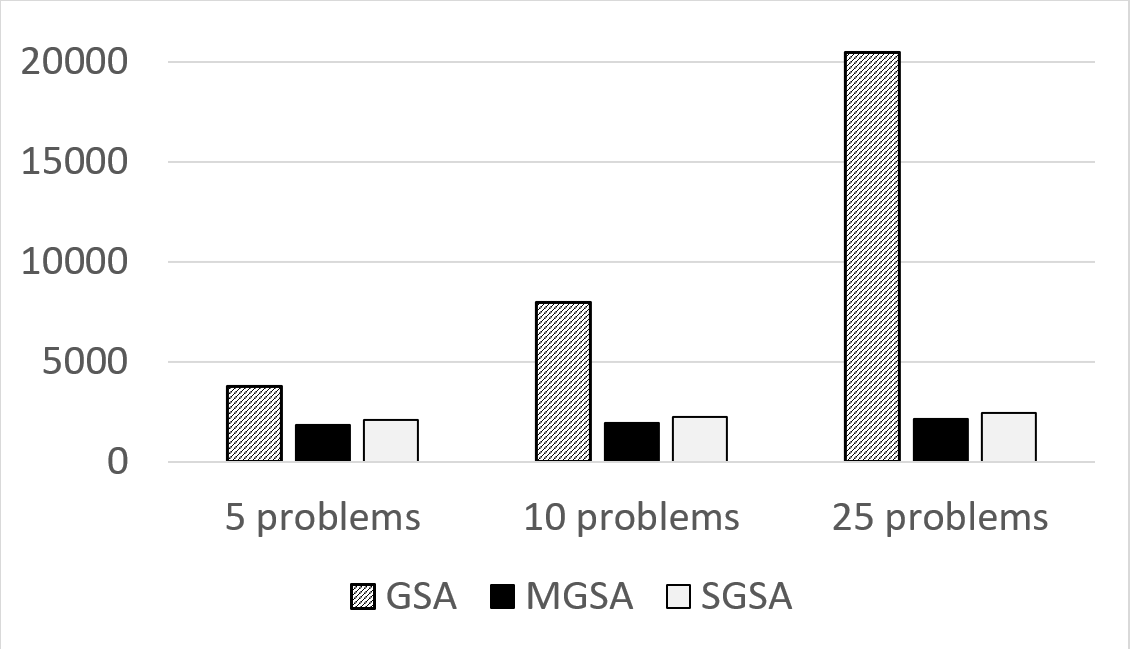
\includegraphics[width=0.7\linewidth]{fig_t2}
  \caption{The average number of iterations for solving bi-criteria two-dimensional MOO problems}
  \label{fig:1}
\end{figure}

The experimental results show that by reusing search information when optimizing 25 functions from the set $\Phi_p (y)$, the total computational iterations can be reduced  by more than 9.5 times without resorting to any additional computational resources. At the same time, the MGSA algorithm performs the least number of iterations (the number of calculations of objective function values), while the SGSA algorithm provides a better approximation of the Pareto domain both in terms of approximation completeness and coverage uniformity. It is also noteworthy that the average number of iterations to optimize one function from the set $\Phi_p (y)$ decreases by more than 4 times as the number of functions in the set $\Phi_p (y)$ increases -- see Table \ref{tab:3}. 

% Please add the following required packages to your document preamble:
% \usepackage{multirow}
\begin{table}[ht]
\centering
\caption{Average number of iterations required to optimize one function from the set $\Phi_p (y)$}
\label{tab:3}
\begin{tabular}{cccc}
\hline
\multirow{2}{*}{\begin{tabular}[c]{@{}c@{}}Number of \\ functions in $\Phi_p (y)$\end{tabular}} & \multicolumn{3}{c}{\begin{tabular}[c]{@{}c@{}}Average number \\ of iterations\end{tabular}} \\
                                                                                        & GSA                           & MGSA                         & SGSA                         \\ \hline
5                                                                                       & 754.4                         & 364.7                        & 418.1                        \\
10                                                                                      & 794.2                         & 195.6                        & 222.4                        \\
25                                                                                      & 818.2                         & 85.4                         & 98.2                         \\ \hline
\end{tabular}
\end{table}

In the third series of numerical experiments, 10 bi-criteria five-dimensional MOO problems were solved, i.e. $N = 5$, $s = 2$. The objective functions of the MOO problems were determined, as before, using the GKLS generator \cite{c43}. When solving the problems, the accuracy $\varepsilon=0.05$ and the reliability $r=5.6$ were used. The results of numerical experiments are presented in Table \ref{tab:4} and Fig. \ref{fig:2}.

\begin{table}[ht]
\centering
\caption{The results of a series of experiments to solve bi-criteria five-dimensional MOO problems}
\label{tab:4}
\begin{tabular}{cccclccclccc}
\hline
\multirow{3}{*}{\begin{tabular}[c]{@{}c@{}}Number of \\ functions in\\ $\Phi_p (y)$\end{tabular}} & \multicolumn{11}{c}{Algorithms}                                                     \\ \cline{2-12} 
                                                                                        & \multicolumn{3}{c}{GSA} &  & \multicolumn{3}{c}{MGSA} &  & \multicolumn{3}{c}{SGSA} \\
                                                                                        & Iters   & HV    & DU    &  & Iters   & HV     & DU    &  & Iters   & HV     & DU    \\ \hline
25                                                                                      & 1030039.6 & 2.440 & 0.543 & & 619755.6 & 2.441 & 0.681 & & 669743.8 & 2.364 & 0.668 \\ 
50                                                                                      & 2061634.2 & 2.502 & 0.572 & & 647508.2 & 2.533 & 0.691 & & 710418.6 & 2.417 & 0.680 \\ 
100                                                                                     & 4104694.4 & 2.504 & 0.686 & & 683410.5 & 2.555 & 0.696 & & 728485.3 & 2.483 & 0.696 \\ \hline
\end{tabular}
\end{table}

\begin{figure}
  \centering
  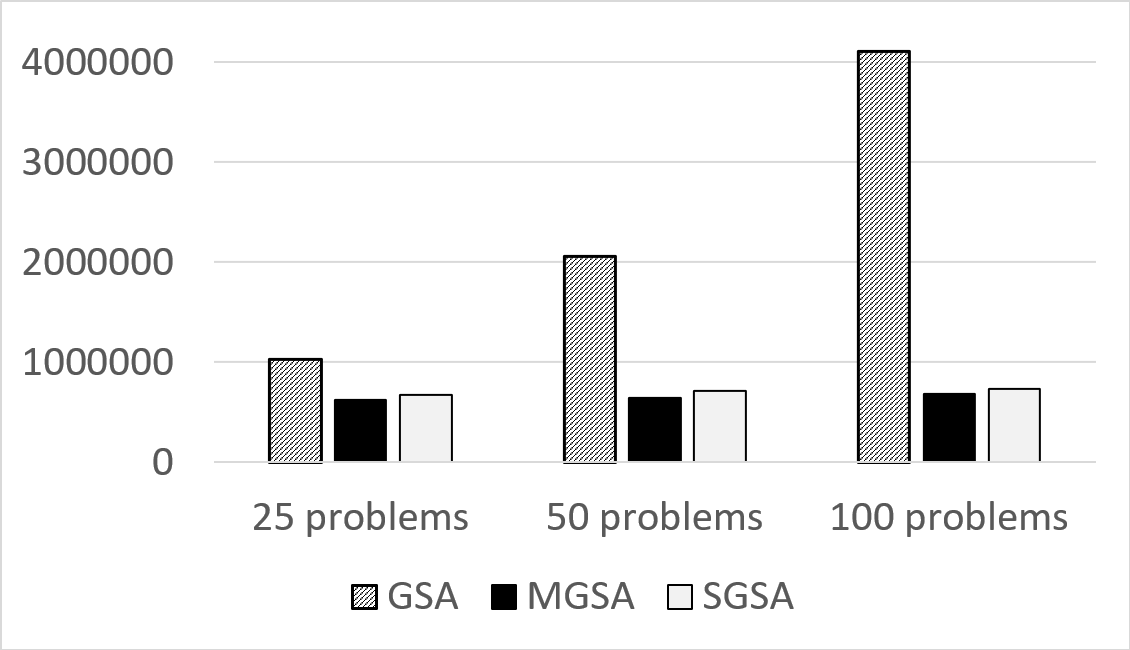
\includegraphics[width=0.7\linewidth]{fig_t5}
  \caption{The average number of iterations for solving bi-criteria five-dimensional MOO problems}
  \label{fig:2}
\end{figure}


The results of our experiments show that with increasing dimensionality of the MOO problems to be solved, the trend that has been identified continues: the amount of computation (the number of global search iterations) is reduced by more than 5.6 times due to reuse of search information, the MGSA algorithm performs the least number of iterations, and the SGSA algorithm provides the best approximation of the Pareto domain.

\section*{Conclusion}

This paper proposes an efficient approach for solving computationally intensive multi-objective optimization problems which require computing several Pareto-optimal decisions. It is also assumed that objective functions may be multiextremal, and computation of function values may require a large amount of calculations. The proposed approach is based on the reduction of multi-objective optimization problems to one-dimensional global optimization problems that can be solved using efficient information-statistical algorithms of global search.  The novelty of the proposed approach consists in the possibility of solving several global optimization problems simultaneously, which allows multiple Pareto-optimal decisions to be obtained. Besides, such approach provides for reuse of the computed search information, which considerably reduces computational effort for solving multi-objective optimization problems. 

The results of numerical experiments show that by using the developed approach it is possible to achieve a significant reduction of computational complexity when solving multi-objective optimization problems. 

It should be noted in conclusion that the proposed approach is promising and requires further research in this area. First of all, it is necessary to continue numerical experiments on solving multi-objective optimization problems with a greater number of objective functions and for higher dimensionality of optimization problems to be solved. The possibility of organizing parallel computations for high-performance systems should also be evaluated.


%
% ---- Bibliography ----
%
% BibTeX users should specify bibliography style 'splncs04'.
% References will then be sorted and formatted in the correct style.
%
\begin{thebibliography}{1}
\providecommand{\url}[1]{\texttt{#1}}
\providecommand{\urlprefix}{URL }
\providecommand{\doi}[1]{https://doi.org/#1}

\bibitem{c1} Miettinen, K.: Nonlinear Multiobjective Optimization. Springer, Boston (1999)
\bibitem{c2} Ehrgott, M.: Multicriteria Optimization, Springer, Berlin (2nd ed., 2010)
\bibitem{c3} Collette, Y., Siarry, P.:  Multiobjective Optimization: Principles and Case Studies (Decision Engineering), Springer, Berlin  (2004)
\bibitem{c4} Marler, R.T., Arora, J.S.: Multi-Objective Optimization: Concepts and Methods for Engineering, VDM Verlag (2009)
\bibitem{c5} Pardalos, P.M., {\v Z}ilinskas, A., {\v Z}ilinskas, J.: Non-Convex Multi-Objective Optimization, Springer (2017)
\bibitem{c6} Marler, R.T., Arora, J.S.: Survey of multi-objective optimization methods for engineering. Struct. Multidiscip. Optim. \textbf{26}, 369--395 (2004)
\bibitem{c7}  Figueira, J., Greco, S., Ehrgott, M., eds.: Multiple Criteria Decision Analysis: State of the Art Surveys. Springer, New York (2005)
\bibitem{c8} Zavadskas, E.K., Turskis, Z., Kildien{\. e}, S.: State of art surveys of overviews on MCDM/MADM methods. Technological and Economic Development of Economy, \textbf{20}, 165--179 (2014)
\bibitem{c9} Hillermeier, C., Jahn, J.: Multiobjective optimization: survey of methods and industrial applications. Surv. Math. Ind. \textbf{11}, 1--42 (2005)
\bibitem{c10} Collette, Y., Siarry, P.: Multiobjective Optimization: Principles and Case Studies. Decision Engineering. Springer, Heidelberg (2011) \doi{10.1007/978-3-662-08883-8}
\bibitem{c11} Eichfelder, G.: Scalarizations for adaptively solving multi-objective optimization problems. Comput. Optim. Appl. \textbf{44}, 249--273 (2009)
\bibitem{c12} Figueira, J., Liefooghe, A., Talbi, E., Wierzbicki, A.: A parallel multiple reference point approach for multi-objective optimization. European Journal of Operational Research \textbf{205}(2), 390--400 (2010) \doi{10.1016/j.ejor.2009.12.027}
\bibitem{c35} Gergel, V.: An unified approach to use of coprocessors of various types for solving global optimization problems. 2nd International Conference on Mathematics and Computers in Sciences and in Industry, 13--18 (2015) \doi{10.1109/MCSI.2015.18}
\bibitem{c36} Gergel, V.P., Kozinov, E.A.: Accelerating multicriterial optimization by the intensive exploitation of accumulated search data. AIP Conference Proceedings \textbf{1776}, 090003 (2016) \doi{10.1063/1.4965367}
\bibitem{c37} Gergel, V., Kozinov, E.: Efficient multicriterial optimization based on intensive reuse of search information. J. Glob. Optim. \textbf{71}(1), 73--90 (2018)
\bibitem{c44} Gergel, V., Kozinov, E., Barkalov, K.: Computationally efficient approach for solving lexicographic multicriteria optimization problems. Optim. Lett. (2020) \doi{10.1007/s11590-020-01668-y}
\bibitem{c13} Zhigljavsky, A.A.: Theory of Global Random Search.  Kluwer Academic Publishers, Dordrecht (1991).
\bibitem{c14} Pint{\' e}r, J.D.: Global Optimization in Action (Continuous and Lipschitz Optimization: Algorithms, Implementations and Applications). Kluwer Academic Publishers, Dortrecht (1996)
\bibitem{c15} Strongin, R., Sergeyev, Ya.: Global Optimization with Non-Convex Constraints. Sequential and Parallel Algorithms. Kluwer Academic Publishers, Dordrecht (2nd ed. 2013, 3rd ed. 2014)
\bibitem{c16} Yang, X.-S.: Nature-inspired Metaheuristic Algorithms. Luniver Press, Frome (2008)
\bibitem{c17} Locatelli, M., Schoen, F.: Global Optimization: Theory, Algorithms, and Applications. SIAM (2013)
\bibitem{c18} Paulavi{\v c}ius, R., {\v Z}ilinskas, J.: Simplicial Global Optimization. Springer, New York (2014).
\bibitem{c19} Floudas, C.A., Pardalos, M.P.: Recent Advances in Global Optimization. Princeton University Press (2016)
\bibitem{c20} Sergeyev, Y.D., Kvasov, D.E.: Deterministic Global Optimization: An Introduction to the Diagonal Approach. Springer, New York (2017) 
\bibitem{c21} Sergeyev, Y.D., Strongin, R.G., Lera, D.: Introduction to Global Optimization Exploiting Space-Filling Curves. Springer (2013)
\bibitem{c22} Piyavskij, S.: An algorithm for finding the absolute extremum of a function. Comput. Math. Math. Phys. \textbf{12}, 57--67 (1972)
\bibitem{c23} Shubert, B.O.: A sequential method seeking the global maximum of a function. SIAM J. Numer. Anal. \textbf{9}, 379--388 (1972)
\bibitem{c24} Strongin, R.G.: Multiextremal minimization. Autom. Remote Control \textbf{7}, 1085--1088 (1970)
\bibitem{c25} Galperin, E.A.: The cubic algorithm. J. Math. Anal. Appl. \textbf{112}, 635--640 (1985)
\bibitem{c26} Breiman, L., Cutler, A.: A deterministic algorithm for global optimization. Math. Program. \textbf{58}, 179--199 (1993)
\bibitem{c27} Baritompa, W.: Accelerations for a variety of global optimization methods. J. Glob. Optim. \textbf{4}, 37--45 (1994)
\bibitem{c28} Gergel, V.P.: A method of using derivatives in the minimization of multiextremum functions. Comput. Math. Math. Phys. \textbf{36}(6), 729--742 (1996)
\bibitem{c29} Sergeyev, Y.D.: Global one-dimensional optimization using smooth auxiliary functions. Math. Program. \textbf{81}, 127--146 (1998)
\bibitem{c30} Sergeyev, Ya.D., Grishagin, V.A.: Sequential and parallel global optimization algorithms. Optim. Methods Softw.\textbf{3}, 111--124 (1994)
\bibitem{c31} Sergeyev, Y.D.: An information global optimization algorithm with local tuning. SIAM J. Optim. \textbf{5}(4), 858--870 (1995)
\bibitem{c32} Sergeyev, Y.D., Grishagin, V.A.: Parallel asynchronous global search and the nested optimization scheme. J. Comput. Anal. Appl. \textbf{3}(2), 123--145 (2001)
\bibitem{c33} Lera, D., Sergeyev, Ya.D.: Deterministic global optimization using space-filling curves and multiple estimates of Lipschitz and Holder constants. Communications in Nonlinear Science and Numerical Simulation \textbf{23}, 328--342 (2015)
\bibitem{c34} Grishagin, V., Israfilov, R., Sergeyev, Y.: Comparative efficiency of dimensionality reduction schemes in global optimization. AIP Conference Proceedings \textbf{1776}, 060011 (2016)
\bibitem{c38} Gergel, V., Barkalov, K., Sysoyev, A.: Globalizer: a novel supercomputer software system for solving time-consuming global optimization problem. Numerical Algebra, Control and Optimization \textbf{8}(1), 47--62 (2018)
\bibitem{c39} {\v Z}ilinskas, A., Zilinskas, J.: Adaptation of a one-step worst-case optimal univariate algorithm of bi-objective Lipschitz optimization to multidimensional problems. Communications in Nonlinear Science and Numerical Simulation \textbf{21}(1-3), 89--98 (2015) \doi{10.1016/j.cnsns.2014.08.025}
\bibitem{c40} Evtushenko, Y., Posypkin, M.: A deterministic algorithm for global multiobjective optimization. Optim. Methods Softw. \textbf{29}(5), 1005--1019 (2014) \doi{10.1080/10556788.2013.854357}
\bibitem{c41} Evtushenko, Y., Posypkin, M.: Method of non-uniform coverages to solve the multicriteria optimization problems with guaranteed accuracy. Autom. Remote Control \textbf{75}(6), 1025--1040 (2014)
\bibitem{c42} Bleuler, S., Laumanns, M., Thiele, L., Zitzler, E.: PISA -- a platform and programming language independent interface for search algorithms. Lecture Notes in Computer Science \textbf{2632}, 494--508 (2003) \doi{10.1007/3-540-36970-8\_35}
\bibitem{c43} Gaviano, M., Kvasov, D.E, Lera, D., Sergeyev, Ya.D.: Software for generation of classes of test functions with known local and global minima for global optimization. ACM Transactions on Mathematical Software \textbf{29}(4), 469--480 (2003)


\end{thebibliography}


%
\end{document}
